\documentclass{article}

\usepackage{stmaryrd}
\usepackage[margin=0.5in]{geometry}
\usepackage{amssymb}
\usepackage{tikz}
\usetikzlibrary{positioning, shadows}

\title{\vspace{1in}Interaction Diagram - Add Version}
\author{Adam Hammes}

% no page number at bottom
\pagenumbering{gobble}

\begin{document}
\maketitle

\begin{center}
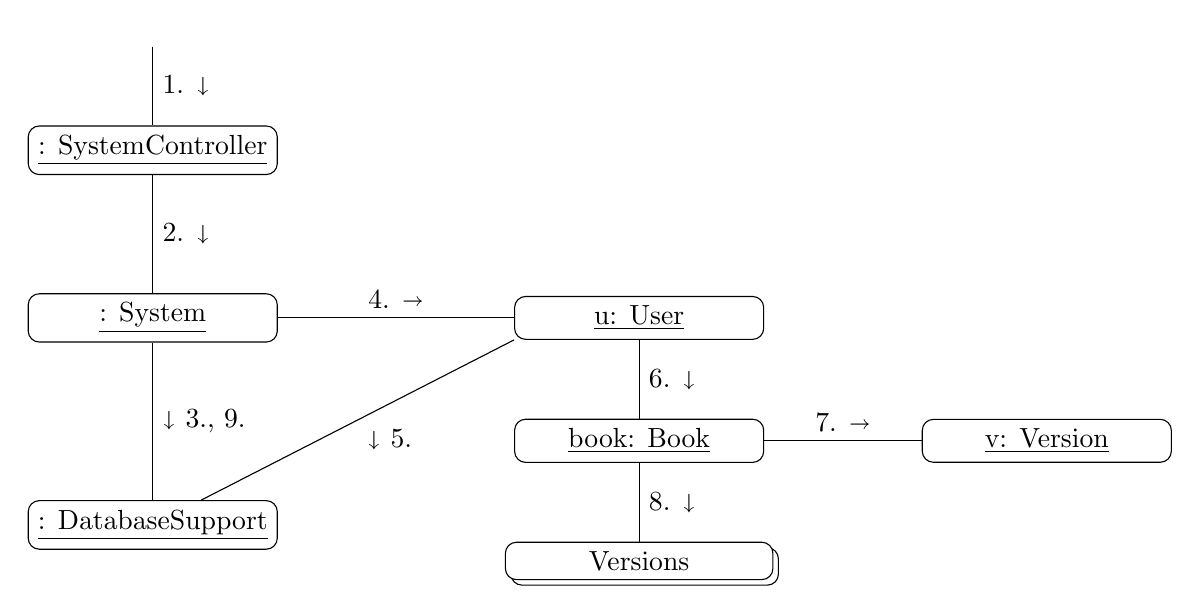
\begin{tikzpicture}[
  auto,
  block/.style = {
    minimum width = 9em,
    rectangle,
    draw=black,
    align=center,
    rounded corners
  },
  multiple/.style = {
    rectangle, draw, rounded corners, fill= white, 
    text width=9em, align= center,
    copy shadow = {
      ,fill=white, draw=black,
      shadow xshift=0.7mm, shadow yshift=-0.7mm
    }
  }
]

\node[] (start)  {};

\node[block, below = of start]         (controller) {\underline{: SystemController}};
\node[block, below = 1.5of controller] (system)     {\underline{: System}};
\node[block, below = 2cm of system]    (database)   {\underline{: DatabaseSupport}};
\node[block, right = 3cm of system]  (user)       {\underline{u: User}};
\node[block, below = of user]    (book)       {\underline{book: Book}};
\node[block, right = 2cm of book]          (version)    {\underline{v: Version}};
\node[multiple, below = of book]          (versions)   {Versions};

\draw (start)      -- (controller) node[midway] {1. $\shortdownarrow$};
\draw (controller) -- (system)     node[midway] {2. $\shortdownarrow$};
\draw (system) -- (database)     node[midway]   {$\shortdownarrow$ 3., 9.};
\draw (system) -- (user)     node[midway]       {4. $\shortrightarrow$};
\draw (user.south west) -- (database) node[midway] {$\shortdownarrow$ 5.};
\draw (user) -- (book) node[midway] {6. $\shortdownarrow$};
\draw (book) -- (version) node[midway] {7. $\shortrightarrow$};
\draw (book) -- (versions) node[midway] {8. $\shortdownarrow$};

\end{tikzpicture}

\vspace{0.5cm}

\begin{enumerate}
  \item \texttt{b:=addVersion(uid:String, bid:String, path:String, type:String):boolean}
  \item \texttt{b:=addVersion(uid:String, bid:String, path:String, type:String):boolean}
  \item \texttt{s:=getUser(uid:String):User}
  \item \texttt{b:=addVersion(bid:String, path:String, type:String):boolean}
  \item \texttt{book:=getBook(bid:String):Book}
  \item \texttt{b:=addVersion(path:String, type:String):boolean}
  \item \texttt{create()}
  \item \texttt{b:=add(v):boolean}
  \item \texttt{b:putUser(u):boolean}
\end{enumerate}
\end{center}

\end{document}
